% === T09 - Memorias y Memoria Caché ===
% David Alejandro Gonzalez Marquez
% fokerman@gmail.com
% https://github.com/fokerman/computingSystemsCourse

\RequirePackage[2020-02-02]{latexrelease}

\documentclass[aspectratio=169]{beamer}
\usepackage{../packages}

\title{\Huge Memorias y Memoria Caché}
\author{David Alejandro González Márquez}
\input{../university}
\date{}

\begin{document}

\begin{frame}[plain]
    \titlepage
    \begin{textblock}{100}(30,80)
    \begin{tcolorbox}[size=small,width=\textwidth,colback={gray!30},title={}]
    \begin{center}
     \scriptsize Clase disponible en: \url{https://github.com/fokerman/computingSystemsCourse}
    \end{center}
    \end{tcolorbox}
    \end{textblock}
%     \begin{textblock}{140}(10,70)
%     \textcolor{rojo}{
%     \textbf{Atención}: La clase será grabada por el anfitrión para su posterior y eventual uso académico dentro de nuestra institución. Su participación en la clase implica brindar su consentimiento para participar en la grabación, aunque pueden mantener su video apagado.}
%     \end{textblock}
\end{frame}

\begin{frame}[fragile,t]{Jerarquía de Memoria}
    \begin{textblock}{100}(18,12) \only<1->{\includegraphics[scale=0.9]{img/jerarquia_memoria-layer1.pdf}} \end{textblock}
    \begin{textblock}{100}(18,12) \only<2->{\includegraphics[scale=0.9]{img/jerarquia_memoria-layer2.pdf}} \end{textblock}
    \begin{textblock}{100}(18,12) \only<3->{\includegraphics[scale=0.9]{img/jerarquia_memoria-layer3.pdf}} \end{textblock}
    \begin{textblock}{100}(18,12) \only<4->{\includegraphics[scale=0.9]{img/jerarquia_memoria-layer4.pdf}} \end{textblock}
    \begin{textblock}{100}(18,12) \only<5->{\includegraphics[scale=0.9]{img/jerarquia_memoria-layer5.pdf}} \end{textblock}
    \begin{textblock}{100}(18,12) \only<6->{\includegraphics[scale=0.9]{img/jerarquia_memoria-layer6.pdf}} \end{textblock}
    \begin{textblock}{100}(18,12) \only<7->{\includegraphics[scale=0.9]{img/jerarquia_memoria-layer7.pdf}} \end{textblock}
    \vspace{6.2cm}
    \begin{center}
    \uncover<8>{Cada uno de los tipos de memoria está implementado con una tecnología diferente.\\}
    \uncover<8>{\textcolor{naranjauca}{A medida que aumentamos la capacidad, se disminuye el costo por bit almacenado.}}
    \end{center}
\end{frame}

\begin{frame}[fragile,t]{Tecnologías de memorias}
    Existen diferentes tipos de memoria
    \begin{itemize}
    \item<1-> \textbf{RAM (Random Access Memory)}\\ Memoria volátil de lectura/escritura.
    \begin{itemize}
    \item \textcolor{naranjauca}{DRAM} (Dynamic Random Access Memory): Construida con capacitores, requiere ser recargada para mantener su estado, muy económica (Memoria Principal).
    \item \textcolor{naranjauca}{SRAM} (Static Random Access Memory): Basada en flip-flops, de costo muy alto, poca densidad, pero muy rápida (Memoria caché).
    \end{itemize}
    \item<2-> \textbf{ROM (Read Only Memory)}\\ No volátil, almacena información esencial para el inicio de un sistema.
    \begin{itemize}
    \item \textcolor{naranjauca}{PROM} (Programmable read-only memory): Se programa una vez y no puede ser borrada.
    \item \textcolor{naranjauca}{EPROM} (Erasable Programmable read only memory): Puede ser borrada y reprogramada mediante la exposición a luz ultravioleta.
    \item \textcolor{naranjauca}{EEPROM} (Electrically erasable programmable read only memory): Puede ser borrada mediante la aplicación de pulsos eléctricos.
    \item \textcolor{naranjauca}{Memoria Flash}: Evolución de las memorias EEPROM, permite escribir por bloques, resultando más económica y densa.
    \end{itemize}
    \end{itemize}
\end{frame}

\begin{frame}[fragile,t]{Memoria Caché}
    Es una memoria intermedia que almacena temporariamente una copia de la información utilizada por la CPU.    
    \begin{textblock}{100}(5,18) \only<1->{\includegraphics[scale=0.795]{img/cpu_cache_memoria-layer1.pdf}} \end{textblock} % CPU
    \begin{textblock}{100}(5,18) \only<1->{\includegraphics[scale=0.795]{img/cpu_cache_memoria-layer2.pdf}} \end{textblock} % Cache
    \begin{textblock}{100}(5,18) \only<1->{\includegraphics[scale=0.795]{img/cpu_cache_memoria-layer3.pdf}} \end{textblock} % Memoria Principal
    \begin{textblock}{100}(5,18) \only<2->{\includegraphics[scale=0.795]{img/cpu_cache_memoria-layer4.pdf}} \end{textblock} % Flecha CPU-Cache
    \begin{textblock}{100}(5,18) \only<2->{\includegraphics[scale=0.795]{img/cpu_cache_memoria-layer5.pdf}} \end{textblock} % Flecha Cache-MP
    \begin{textblock}{100}(5,18) \only<5->{\includegraphics[scale=0.795]{img/cpu_cache_memoria-layer6.pdf}} \end{textblock} % Linea CPU-Cache
    \begin{textblock}{100}(5,18) \only<3->{\includegraphics[scale=0.795]{img/cpu_cache_memoria-layer7.pdf}} \end{textblock} % Linea Cache-MP
    \begin{textblock}{100}(5,18) \only<4->{\includegraphics[scale=0.795]{img/cpu_cache_memoria-layer8.pdf}} \end{textblock} % Organizacion Memoria
    \begin{textblock}{100}(5,18) \only<7->{\includegraphics[scale=0.795]{img/cpu_cache_memoria-layer9.pdf}} \end{textblock} % Politica Remplazo
    \begin{textblock}{100}(5,18) \only<7->{\includegraphics[scale=0.795]{img/cpu_cache_memoria-layer10.pdf}} \end{textblock} % Politica Escritura
    \begin{textblock}{100}(5,18) \only<6->{\includegraphics[scale=0.795]{img/cpu_cache_memoria-layer11.pdf}} \end{textblock} % Localidad Espacial y temporal
    \vspace{4.3cm}
    \uncover<2->{Es un componente fundamental para reducir la \textbf{latencia} a la memoria principal.\\}
    \uncover<6->{Basa su funcionamiento en el principio de \textbf{localidad} espacial y temporal.\\}
    \uncover<7->{Implementa una estructura propia con \textbf{políticas de remplazo} y \textbf{escritura}.\\}
    \uncover<8->{Debe ser \textbf{transparente} para la CPU.\\}
\end{frame}

\begin{frame}{¿Cómo funciona la Memoria Caché?}
    \begin{textblock}{100}(14,10) \only<1->{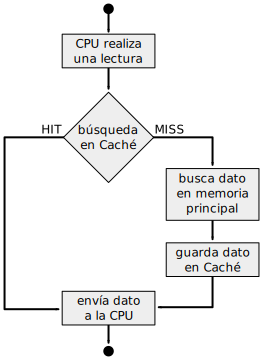
\includegraphics[scale=0.7]{img/cache_funcionamiento.pdf}} \end{textblock}
    \begin{textblock}{76}(76,20)
    Eventos tras un acceso
    \vskip 2pt
    \begin{itemize}
        \item \textbf{Hit:} El dato solicitado se encuentra en caché
        \item \textbf{Miss:} En caso contrario
    \end{itemize}
    \vskip 9pt
    Métricas
    \vskip 2pt
    \begin{itemize}
        \item $\textbf{Hit\ Rate}\ =\ \frac{\#hits}{\#pedidos}$
        \item $\textbf{Miss\ Rate}\ =\ \frac{\#miss}{\#pedidos}$
    \end{itemize}
    \vskip 15pt
    \begin{block}{Objetivo}
    Lograr que el \textcolor{naranjauca}{hit rate} sea lo más alto posible.
    \end{block}
    \end{textblock}
\end{frame}

\begin{frame}{Localidad Espacial y Localidad Temporal}
    Durante un \emph{miss}, la memoria caché solicita a la memoria principal el dato buscado junto con los datos vecinos. De esta forma, anticipa los futuros pedidos.
    \bigskip
    \begin{itemize}
    \item \textbf{Localidad Espacial}:\\
    Si se pide un dato en memoria, es altamente probable que a continuación se pida también otro dato que esté próximo a él en memoria. Ejemplos: ejecución secuencial, recorrido de arrays, etc.
    \vskip 15pt
    \item \textbf{Localidad Temporal}:\\
    Si se pide un dato en memoria, es altamente probable que este vuelva a ser reutilizado en un futuro inmediato. Ejemplos: variables, ciclos, etc.
    \end{itemize}
\end{frame}

\begin{frame}{Tipos de Caché}
    \begin{textblock}{80}(5,18)
    \begin{itemize}
    \item<1-> \textbf{Totalmente Asociativa}:\\ Cada bloque en caché puede contener cualquier dato de la memoria principal.\\
    \vskip 15pt
    \item<2-> \textbf{Correspondencia Directa}:\\ Los bloques de caché almacenan direcciones específicas de memoria principal.\\
    \vskip 15pt
    \item<3-> \textbf{Asociativa por Conjuntos}:\\ Los bloques de caché se dividen en conjuntos y cada uno puede almacenar un conjunto de direcciones específicas de memoria principal.\\
    \end{itemize}
    \end{textblock}
    \begin{textblock}{80}(100,15)
    \only<1->{\includegraphics[scale=0.8]{img/memorias_cache_ilustracion-layer1.pdf}\\}
    \vspace{1.1cm}
    \only<2->{\includegraphics[scale=0.8]{img/memorias_cache_ilustracion-layer2.pdf}\\}
    \vspace{1.1cm}
    \only<3->{\includegraphics[scale=0.8]{img/memorias_cache_ilustracion-layer3.pdf}}
    \end{textblock}    
\end{frame}

\begin{frame}{Políticas}
    \textcolor{naranjauca}{Política de reemplazo}
    \begin{itemize}
    \item \textbf{First In First Out} (FIFO):\\ El primer dato en entrar es el primero en ser descartado.
    \vskip 5pt
    \item \textbf{Least Recently Used} (LRU):\\ Se descarta el dato menos recientemente usado.
    \vskip 5pt
    \item \textbf{Least Frequently Used} (LFU):\\ Se descarta el bloque menos frecuentemente usado.
    \end{itemize}
    \bigskip
    \pause
    \textcolor{naranjauca}{Política de escritura}
    \begin{itemize}
    \item \textbf{Write-through}:\\ Se escribe en caché y en memoria al mismo tiempo.
    \vskip 5pt
    \item \textbf{Write-back}:\\ Se escribe en memoria principal cuando se desaloja el dato de caché.
    \end{itemize}
\end{frame}

\begin{frame}{Tipos de fallos}
    \begin{textblock}{80}(5,18)
    \begin{itemize}
    \item<1-> \textbf{Forzosos} (Compulsory):\\ En el primer acceso este no se encuentra en la caché (primera referencia).
    \vskip 25pt
    \item<2-> \textbf{Capacidad} (Capacity):\\ La caché no puede contener todos los bloques necesarios durante la ejecución de un programa.
    \vskip 25pt
    \item<3-> \textbf{Conflicto} (Conflict):\\ Diferentes bloques deben ir necesariamente al mismo conjunto o línea (fallos de colisión).
    \end{itemize}
    \end{textblock}
    \begin{textblock}{80}(100,10)
    \only<1->{\includegraphics[scale=0.8]{img/memorias_cache_fallas-layer1.pdf}\\}
    \vspace{0.9cm}
    \only<2->{\includegraphics[scale=0.8]{img/memorias_cache_fallas-layer2.pdf}\\}
    \vspace{0.9cm}
    \only<3->{\includegraphics[scale=0.8]{img/memorias_cache_fallas-layer3.pdf}}
    \end{textblock}
\end{frame}

\begin{frame}{Estructura de una Caché}
    \begin{textblock}{80}(8,13) \only<1->{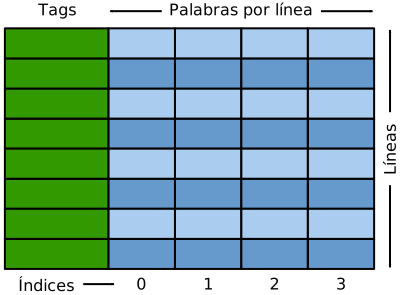
\includegraphics[scale=0.65]{img/cache_estructura.pdf}} \end{textblock}
    \begin{textblock}{80}(95,10) \only<1->{\includegraphics[scale=0.85]{img/tag-linea-indice-layer1.pdf}} \end{textblock}
    \begin{textblock}{55}(95,33)
    \normalsize \textbf{Índice}: \small \textcolor{naranjauca}{log$_2$($N$)} bits.\\
    \normalsize Indica la posición del dato dentro de una línea.\\
    \vskip 10pt
    \normalsize \textbf{Línea}: \small \textcolor{naranjauca}{log$_2$($K$/V)} bits.\\
    \normalsize Mínima unidad de almacenamiento en la memoria caché.\\
    \vskip 10pt
    \normalsize \textbf{Tag}: \small \textcolor{naranjauca}{$M-$Línea$-$Índice} bits.\\
    \normalsize Identificador del dato en memoria principal.\\
    \end{textblock}
    \begin{textblock}{80}(10,72)
    \textbf{Memoria Principal}: \textcolor{naranjauca}{$2^{M}$} bytes, direccionable a byte.\\
    \textbf{Caché}: \textcolor{naranjauca}{$K$} l\'ineas de \textcolor{naranjauca}{$N$} bytes y \textcolor{naranjauca}{V} vías.
    \end{textblock}
\end{frame}

\begin{frame}[fragile,t]{Ejemplos de tipos de memorias caché}
    Para comprender el funcionamiento de cada uno de los tipos de memorias caché,\\
    vamos a armar un ejemplo para cada tipo:\\
    \bigskip
    Considerar una \textbf{memoria principal de 64} bytes\\
    y una \textbf{memoria caché de 16} bytes\\
    con las siguientes características:\\
    \vskip 5pt
    \begin{itemize}
    \item[A] \textcolor{naranjauca}{\textbf{Totalmente Asociativa}}\\ 4 líneas, 4 bytes por línea
    \vskip 10pt
    \item[B] \textcolor{naranjauca}{\textbf{Correspondencia Directa}}\\ 4 líneas, 4 bytes por línea
    \vskip 10pt
    \item[C] \textcolor{naranjauca}{\textbf{Asociativa por Conjuntos}}\\ 2 vías (es decir, 2 líneas por conjunto), 2 conjuntos, 4 bytes por línea
    \end{itemize}
\end{frame}

\begin{frame}{A - \textbf{Totalmente Asociativa}}
    \begin{textblock}{80}(25,13) \only<1->{\includegraphics[scale=0.85]{img/caches_tipos_ejemplos-layer7.pdf}} \end{textblock} % Flecha
    \begin{textblock}{80}(25,13) \only<1->{\includegraphics[scale=0.85]{img/caches_tipos_ejemplos-layer1.pdf}} \end{textblock} % FA
    \begin{textblock}{80}(25,13) \only<2->{\includegraphics[scale=0.85]{img/caches_tipos_ejemplos-layer4.pdf}} \end{textblock} % FA Ejemplo
    \begin{textblock}{80}(25,13) \only<3->{\includegraphics[scale=0.85]{img/caches_tipos_ejemplos-layer8.pdf}} \end{textblock} % FA
    \begin{textblock}{80}(25,13) \only<4->{\includegraphics[scale=0.85]{img/caches_tipos_ejemplos-layer9.pdf}} \end{textblock} % FA
    \begin{textblock}{80}(25,13) \only<5->{\includegraphics[scale=0.85]{img/caches_tipos_ejemplos-layer10.pdf}} \end{textblock} % FA
    \begin{textblock}{80}(25,13) \only<6->{\includegraphics[scale=0.85]{img/caches_tipos_ejemplos-layer11.pdf}} \end{textblock} % FA
\end{frame}

\begin{frame}{B - \textbf{Correspondencia Directa}}
    \begin{textblock}{80}(25,13) \only<1->{\includegraphics[scale=0.85]{img/caches_tipos_ejemplos-layer7.pdf}} \end{textblock} % Flecha
    \begin{textblock}{80}(25,13) \only<1->{\includegraphics[scale=0.85]{img/caches_tipos_ejemplos-layer2.pdf}} \end{textblock} % MD
    \begin{textblock}{80}(25,13) \only<2->{\includegraphics[scale=0.85]{img/caches_tipos_ejemplos-layer5.pdf}} \end{textblock} % MD Ejemplo
    \begin{textblock}{80}(25,13) \only<3->{\includegraphics[scale=0.85]{img/caches_tipos_ejemplos-layer12.pdf}} \end{textblock} % MD
    \begin{textblock}{80}(25,13) \only<4->{\includegraphics[scale=0.85]{img/caches_tipos_ejemplos-layer13.pdf}} \end{textblock} % MD
    \begin{textblock}{80}(25,13) \only<5->{\includegraphics[scale=0.85]{img/caches_tipos_ejemplos-layer14.pdf}} \end{textblock} % MD
    \begin{textblock}{80}(25,13) \only<6->{\includegraphics[scale=0.85]{img/caches_tipos_ejemplos-layer15.pdf}} \end{textblock} % MD
\end{frame}

\begin{frame}{C - \textbf{Asociativa por Conjuntos}}
    \begin{textblock}{80}(25,13) \only<1->{\includegraphics[scale=0.85]{img/caches_tipos_ejemplos-layer7.pdf}} \end{textblock} % Flecha
    \begin{textblock}{80}(25,13) \only<1->{\includegraphics[scale=0.85]{img/caches_tipos_ejemplos-layer3.pdf}} \end{textblock} % AC
    \begin{textblock}{80}(25,13) \only<2->{\includegraphics[scale=0.85]{img/caches_tipos_ejemplos-layer6.pdf}} \end{textblock} % AC Ejemplo
    \begin{textblock}{80}(25,13) \only<3->{\includegraphics[scale=0.85]{img/caches_tipos_ejemplos-layer16.pdf}} \end{textblock} % AC
    \begin{textblock}{80}(25,13) \only<4->{\includegraphics[scale=0.85]{img/caches_tipos_ejemplos-layer17.pdf}} \end{textblock} % AC
    \begin{textblock}{80}(25,13) \only<5->{\includegraphics[scale=0.85]{img/caches_tipos_ejemplos-layer18.pdf}} \end{textblock} % AC
    \begin{textblock}{80}(25,13) \only<6->{\includegraphics[scale=0.85]{img/caches_tipos_ejemplos-layer19.pdf}} \end{textblock} % AC
\end{frame}

\begin{frame}[t]
    \frametitle{Ejemplos - Correspondencia Directa}
    \small 
    \textbf{Memoria Principal} $2^{20}$ bytes, direccionable a byte.\\
    \textbf{Caché}  $32$ l\'ineas de $16$ bytes cada una.\\
    \bigskip
    \textcolor{naranjauca}{Índice} $=$ log$_2$(16) $=$ \textbf{4 bits}\\
    \textcolor{naranjauca}{Línea} $=$ log$_2$(32) $=$ \textbf{5 bits}\\
    \textcolor{naranjauca}{Tags} $=$ $20$ $-$ $4$ $-$ $5$ $=$ \textbf{11 bits}\\
    \bigskip
    \textbf{?`Está cargada en caché la línea donde se encuentra el dato de la direcci\'on \texttt{C34A6}?}\\
    \vskip 5pt
    \small
    Paso la dirección a binario:\\
    \vskip -15pt
    \begin{equation*}
    \text{}\frac{C}{1100} \frac{3}{0011} \frac{4}{0100} \frac{A}{1010} \frac{6}{0110}
    \end{equation*}
    Separo seg\'un los campos \textbf{tag} 11 $bits$, \textbf{l\'inea} 5 $bits$, \textbf{\'indice} 4 $bits$:\\
    \vskip -5pt
    \begin{equation*}
    \text{}\frac{61A}{110\text{ }0001\text{ }1010} \frac{A}{0\text{ }1010} \frac{6}{0110}
    \end{equation*}
    Si en la \textbf{línea} número \texttt{0xA} se encuentrá el \emph{tag} n\'umero \texttt{0x61A},\\
    entonces la línea se encuentra en la memoria caché.
\end{frame}

\begin{frame}[t]
    \frametitle{Ejemplos - Asociativa por Conjuntos}
    \small 
    \textbf{Memoria Principal} $1$ MB, direccionable a byte.\\
    \textbf{Caché}  $32$ l\'ineas de $64$ bytes cada una, 2 v\'ias.\\
    \bigskip
    \textcolor{naranjauca}{Índice} $=$ log$_2$(64) $=$ \textbf{6 bits}\\
    \textcolor{naranjauca}{Línea} $=$ log$_2$(32/2) $=$ \textbf{4 bits}\\
    \textcolor{naranjauca}{Tags} $=$ $20$ $-$ $4$ $-$ $6$ $=$ \textbf{10 bits}\\
    \bigskip
    \textbf{?`Está cargada en caché la línea donde se encuentra el dato de la direcci\'on \texttt{C34A6}?}\\
    \vskip 5pt
    \small
    Paso la dirección a binario:\\
    \vskip -15pt
    \begin{equation*}
    \text{}\frac{C}{1100} \frac{3}{0011} \frac{4}{0100} \frac{A}{1010} \frac{6}{0110}
    \end{equation*}
    Separo seg\'un los campos \textbf{tag} 10 $bits$, \textbf{l\'inea} 4 $bits$, \textbf{\'indice} 6 $bits$:\\
    \vskip -5pt
    \begin{equation*}
    \text{}\frac{30D}{11\text{ }0000\text{ }1101} \frac{2}{0010} \frac{26}{10\text{ }0110}
    \end{equation*}
    Si en el \textbf{conjunto} número \texttt{0x2} se encuentrá el \emph{tag} n\'umero \texttt{0x30D},\\
    entonces la línea se encuentra en la memoria caché.
\end{frame}

\begin{frame}[t]
\frametitle{Ejemplos - Asociativa por Conjuntos}
    \small
    \textbf{Memoria Principal} $1$ MB, direccionable a byte.\\
    \textbf{Caché}  $32$ l\'ineas de $64$ bytes cada una, 2 v\'ias, \textcolor{verdeuca}{\textbf{política de remplazo FIFO}}.\\ 
    \bigskip
    Suponiendo accesos a memoria de dos bytes, indicar el \textbf{hit-rate} de las siguientes lecturas a memoria, indicando en cada paso qué datos guarda la memoria caché:\\
    \begin{center}
    \texttt{0xC34A6}\\
    \texttt{0xC38AB}\\
    \texttt{0xC3480}\\
    \texttt{0xC34D4}\\
    \texttt{0xC34FF}\\
    \texttt{0xC34BF}\\
    \texttt{0x00090}
    \end{center}
    \textcolor{naranjauca}{Índice} $=$ log$_2$(64) $=$ \textbf{6 bits}\\
    \textcolor{naranjauca}{Línea} $=$ log$_2$(32/2) $=$ \textbf{4 bits}\\
    \textcolor{naranjauca}{Tags} $=$ $20$ $-$ $4$ $-$ $6$ $=$ \textbf{10 bits}\\
\end{frame}

\begin{frame}[t]
\frametitle{Ejemplos - Asociativa por Conjuntos}
    \scriptsize
    \textbf{Memoria Principal} $1$ MB, direccionable a byte.\\
    \textbf{Caché}  $32$ l\'ineas de $64$ bytes cada una, 2 v\'ias, \textcolor{verdeuca}{\textbf{Politica de remplazo FIFO}}.\\ 
    Indicar el \textbf{hit-rate} de las siguientes lecturas a memoria de 2 bytes, indicando en cada paso qué datos guarda la memoria caché:\\
    \scriptsize
    \vskip 5pt
    \begin{tabular}{|c|c|c|c|c|l|l|}
    \hline
        Direcci\'on   & Tag                &  Set               & \'Indice          & Resultado           & Estado Caché                    & Notas\\ \hline
        C34A6         & \uncover<6->{30D}  &  \uncover<6->{2}   & \uncover<6->{26}  & \uncover<7->{Miss}  & \uncover<7->{\{2:30D\}}         & \uncover<7->{cargu\'e 2:30D}                                         \\
    $\uncover<3->{30D \above 0.4pt} \uncover<2->{1100\text{ }0011\text{ }01}$ $\uncover<4->{2 \above 0.4pt} \uncover<2->{00\text{ }10}$ $\uncover<5->{26 \above 0.4pt} \uncover<2->{10\text{ }0110}$   & & & & & & \\[0.05cm] \hline
        C38AB         & \uncover<10->{30E} &  \uncover<10->{2}  & \uncover<10->{2B} & \uncover<11->{Miss} & \uncover<11->{\{2:30D, 2:30E\}} & \uncover<11->{cargu\'e 2:30E}                                        \\
    $\uncover<9->{30E \above 0.4pt} \uncover<8->{1100\text{ }0011\text{ }10}$ $\uncover<9->{2 \above 0.4pt} \uncover<8->{00\text{ }10}$ $\uncover<9->{2B \above 0.4pt} \uncover<8->{10\text{ }1011}$   & & & & & & \\[0.05cm] \hline
        C3480         & \uncover<13->{30D} &  \uncover<13->{2}  & \uncover<13->{00} & \uncover<14->{Hit}  & \uncover<14->{\{2:30D, 2:30E\}} &                                                                      \\
    \uncover<12->{$30D \above 0.4pt 1100\text{ }0011\text{ }01$ $2 \above 0.4pt 00\text{ }10$ $00 \above 0.4pt 00\text{ }0000$}                                                                        & & & & & & \\[0.05cm] \hline
        C34D4         & \uncover<16->{30D} &  \uncover<16->{3}  & \uncover<16->{14} & \uncover<17->{Miss} & \uncover<17->{\{2:30D, 2:30E\}} & \uncover<17->{cargu\'e 3:30D}                                        \\
    \uncover<15->{$30D \above 0.4pt 1100\text{ }0011\text{ }01$ $3 \above 0.4pt 00\text{ }11$ $14 \above 0.4pt 01\text{ }0100$}                                                                        & & & & & \uncover<17->{\{3:30D\}} & \\[0.05cm] \hline
        C34FF         & \uncover<19->{30D} &  \uncover<19->{3}  & \uncover<19->{3F} & \uncover<20->{Miss} & \uncover<21->{\{2:30D, 2:30E\}} & \uncover<21->{acc. desalineado;}                                                              \\
    \uncover<18->{$30D \above 0.4pt 1100\text{ }0011\text{ }01$ $3 \above 0.4pt 00\text{ }11$ $3F \above 0.4pt 11\text{ }1111$}                                                                        & & & & & \uncover<21->{\{3:30D\}} & \uncover<21->{cargu\'e 4:30D} \\
                      &                    &                    &                   &                     & \uncover<21->{\{4:30D\}}        &                                                                                                                             \\ \hline
        C34BF         & \uncover<22->{30D} &  \uncover<22->{2}  & \uncover<22->{3F} & \uncover<23->{Hit}  & \uncover<23->{\{2:30D, 2:30E\}} & \uncover<23->{acc. desalineado;}                                                                                            \\ 
    \uncover<22->{$30D \above 0.4pt 1100\text{ }0011\text{ }01$ $2 \above 0.4pt 00\text{ }10$ $3F \above 0.4pt 11\text{ }1111$}                                                                        & & & & & \uncover<23->{\{3:30D\}} & \uncover<23->{tengo ambas}    \\
                      &                    &                    &                   &                     & \uncover<23->{\{4:30D\}}        &                                                                                                                             \\ \hline
        00090         & \uncover<24->{000} &  \uncover<24->{2}  & \uncover<24->{10} & \uncover<25->{Miss} & \uncover<25->{\{2:30E, 2:000\}} & \uncover<25->{desaloj\'e 2:30D}                                                                                             \\
    \uncover<24->{$000 \above 0.4pt 0000\text{ }0000\text{ }00$ $2 \above 0.4pt 00\text{ }10$ $10 \above 0.4pt 01\text{ }0000$}                                                                        & & & & & \uncover<25->{\{3:30D\}} &                               \\
                      &                    &                    &                   &                     & \uncover<25->{\{4:30D\}}        &                                                                                                                             \\ \hline
    \end{tabular}    
    \begin{textblock}{80}(130,78)
    \uncover<26->{\emph{Hit rate} =} \uncover<27->{$\frac{2}{7}$ $\approx$ 0.29\%}
    \end{textblock}
\end{frame}

% - Memoria caché en la vida real
% - Ejemplo 286
% - Ejemplo Pentium 4
% - Ejemplo I7

\begin{frame}[fragile]
    \frametitle{Bibliografía}
    \begin{itemize}
     \setlength\itemsep{0.5cm}
    \item[-] \small Tanenbaum, “Organización de Computadoras. Un Enfoque Estructurado”, 4ta Edición, 2000.\\
    \begin{itemize}
     \item \textbf{Seleccionados}\\
     \begin{itemize}
      \item 2.2.5 Memoria Caché - Páginas 65 - 67
      \item 2.3 Memoria Secundaria - Páginas 68 - 69
      \item 3.3.6 Las memorias RAM y las ROM - Páginas 152 - 154
      \item 4.5 Mejoramiento del desempeño - Páginas 264 - 270
     \end{itemize}
    \end{itemize}
    \item[-] \small Null, “Essentials of Computer Organization and Architecture”, 5th Edition, 2018.\\
    \begin{itemize}
    \item \textbf{Chapter 6 - Memory}
     \begin{itemize}
        \item 6.2 Types of Memory
        \item 6.3 The Memory Hierarchy
        \item 6.4 Cache Memory
     \end{itemize}
    \end{itemize}
%     \item[-] \small Silberschatz, “Fundamentos de Sistemas Operativos”, 7ma Edición, 2006.\\
%     \item[-] \small Tanenbaum, “Modern Operating Systems”, 4th Edition, 2015.\\
    \end{itemize}
\end{frame}

\begin{frame}[plain]
    \begin{center}
    \vspace{2cm}
    \huge ¡Gracias!\\
    \vspace{2cm}
%     \normalsize Recuerden leer los comentarios adjuntos\\ en cada clase por aclaraciones.
    \end{center}
\end{frame}

\end{document}

